\documentclass[a4paper]{article}
\addtolength{\hoffset}{-2.25cm}
\addtolength{\textwidth}{4.5cm}
\addtolength{\voffset}{-3.25cm}
\addtolength{\textheight}{5cm}
\setlength{\parskip}{0pt}
\setlength{\parindent}{0in}

\usepackage[square,sort,comma,numbers]{natbib}
\usepackage{blindtext} % Package to generate dummy text
\usepackage{charter} % Use the Charter font
\usepackage[utf8]{inputenc} % Use UTF-8 encoding
\usepackage{microtype} % Slightly tweak font spacing for aesthetics
\usepackage{amsthm, amsmath, amssymb} % Mathematical typesetting
\usepackage{float} % Improved interface for floating objects
\usepackage{hyperref} % For hyperlinks in the PDF
\usepackage{graphicx, multicol} % Enhanced support for graphics
\usepackage{xcolor} % Driver-independent color extensions
\usepackage{pseudocode} % Environment for specifying algorithms in a natural way
\usepackage[mmddyy]{datetime} % Uses YEAR-MONTH-DAY format for dates

\usepackage{fancyhdr} % Headers and footers
\pagestyle{fancy} % All pages have headers and footers
\fancyhead{}\renewcommand{\headrulewidth}{0pt} % Blank out the default header
\fancyfoot[L]{} % Custom footer text
\fancyfoot[C]{} % Custom footer text
\fancyfoot[R]{\thepage} % Custom footer text
\newcommand{\note}[1]{\marginpar{\scriptsize \textcolor{red}{#1}}} % Enables comments in red on margin

\DeclareMathOperator*{\argmin}{arg\,min}

%----------------------------------------------------------------------------------------

\newcommand{\yourname}{Balthazar Neveu}
\newcommand{\youremail}{balthazarneveu@gmail.com}
\newcommand{\assignmentnumber}{7}

\begin{document}

\fancyhead[C]{}
\hrule \medskip
\begin{minipage}{0.295\textwidth} 
\raggedright
\footnotesize
\yourname \hfill\\
\youremail
\end{minipage}
\begin{minipage}{0.4\textwidth} 
\centering 
\large 
Lab session \# \assignmentnumber\\ 
\normalsize 
ALTEGRAD 2023\\ 
\end{minipage}
\begin{minipage}{0.295\textwidth} 
\raggedleft
\today\hfill\\
\end{minipage}
\medskip\hrule 
\bigskip


\section*{Code}

More info:
\href{https://github.com/balthazarneveu/MVA23_ALTEGRAD/#readme}{MVA ALTEGRAD Balthazar Neveu on Github}

\section*{DeepSets: Learn to add \textit{(add to learn...)}}
\section*{Question 1 : LSTM are not permutation invariant, therefore not recommended for sets processing}
Permutation invariance refers to the property where the model's output does not change if the order of the input data is changed. For instance, in a permutation invariant model, the input sequence [1, 2, 3] would yield the same output as [3, 2, 1]. Permuation invaraiance is a desirable property to deal with sets.
\newline
Long Short-Term Memory (LSTM) models are not permutation invariant. LSTM process sequential data in a recurrent fashion and maintain a kind of memory. Order matters for natural language processing or time series but not for sets. 

LSTM are therefore not suited for sets processing.
\newline



We confirm this with the figure \ref{fig:performances_deepset_lstm_evolution} from task 7.
Please note that this figure may be a bit misleading  as the results of deepSet look almost too good to be true (100\% accuracy), which is why I also report the accuracies of Deepset and LSTM while training \ref{fig:performances_deepset_lstm_evolution}.

\begin{figure}[h]
    \centering
    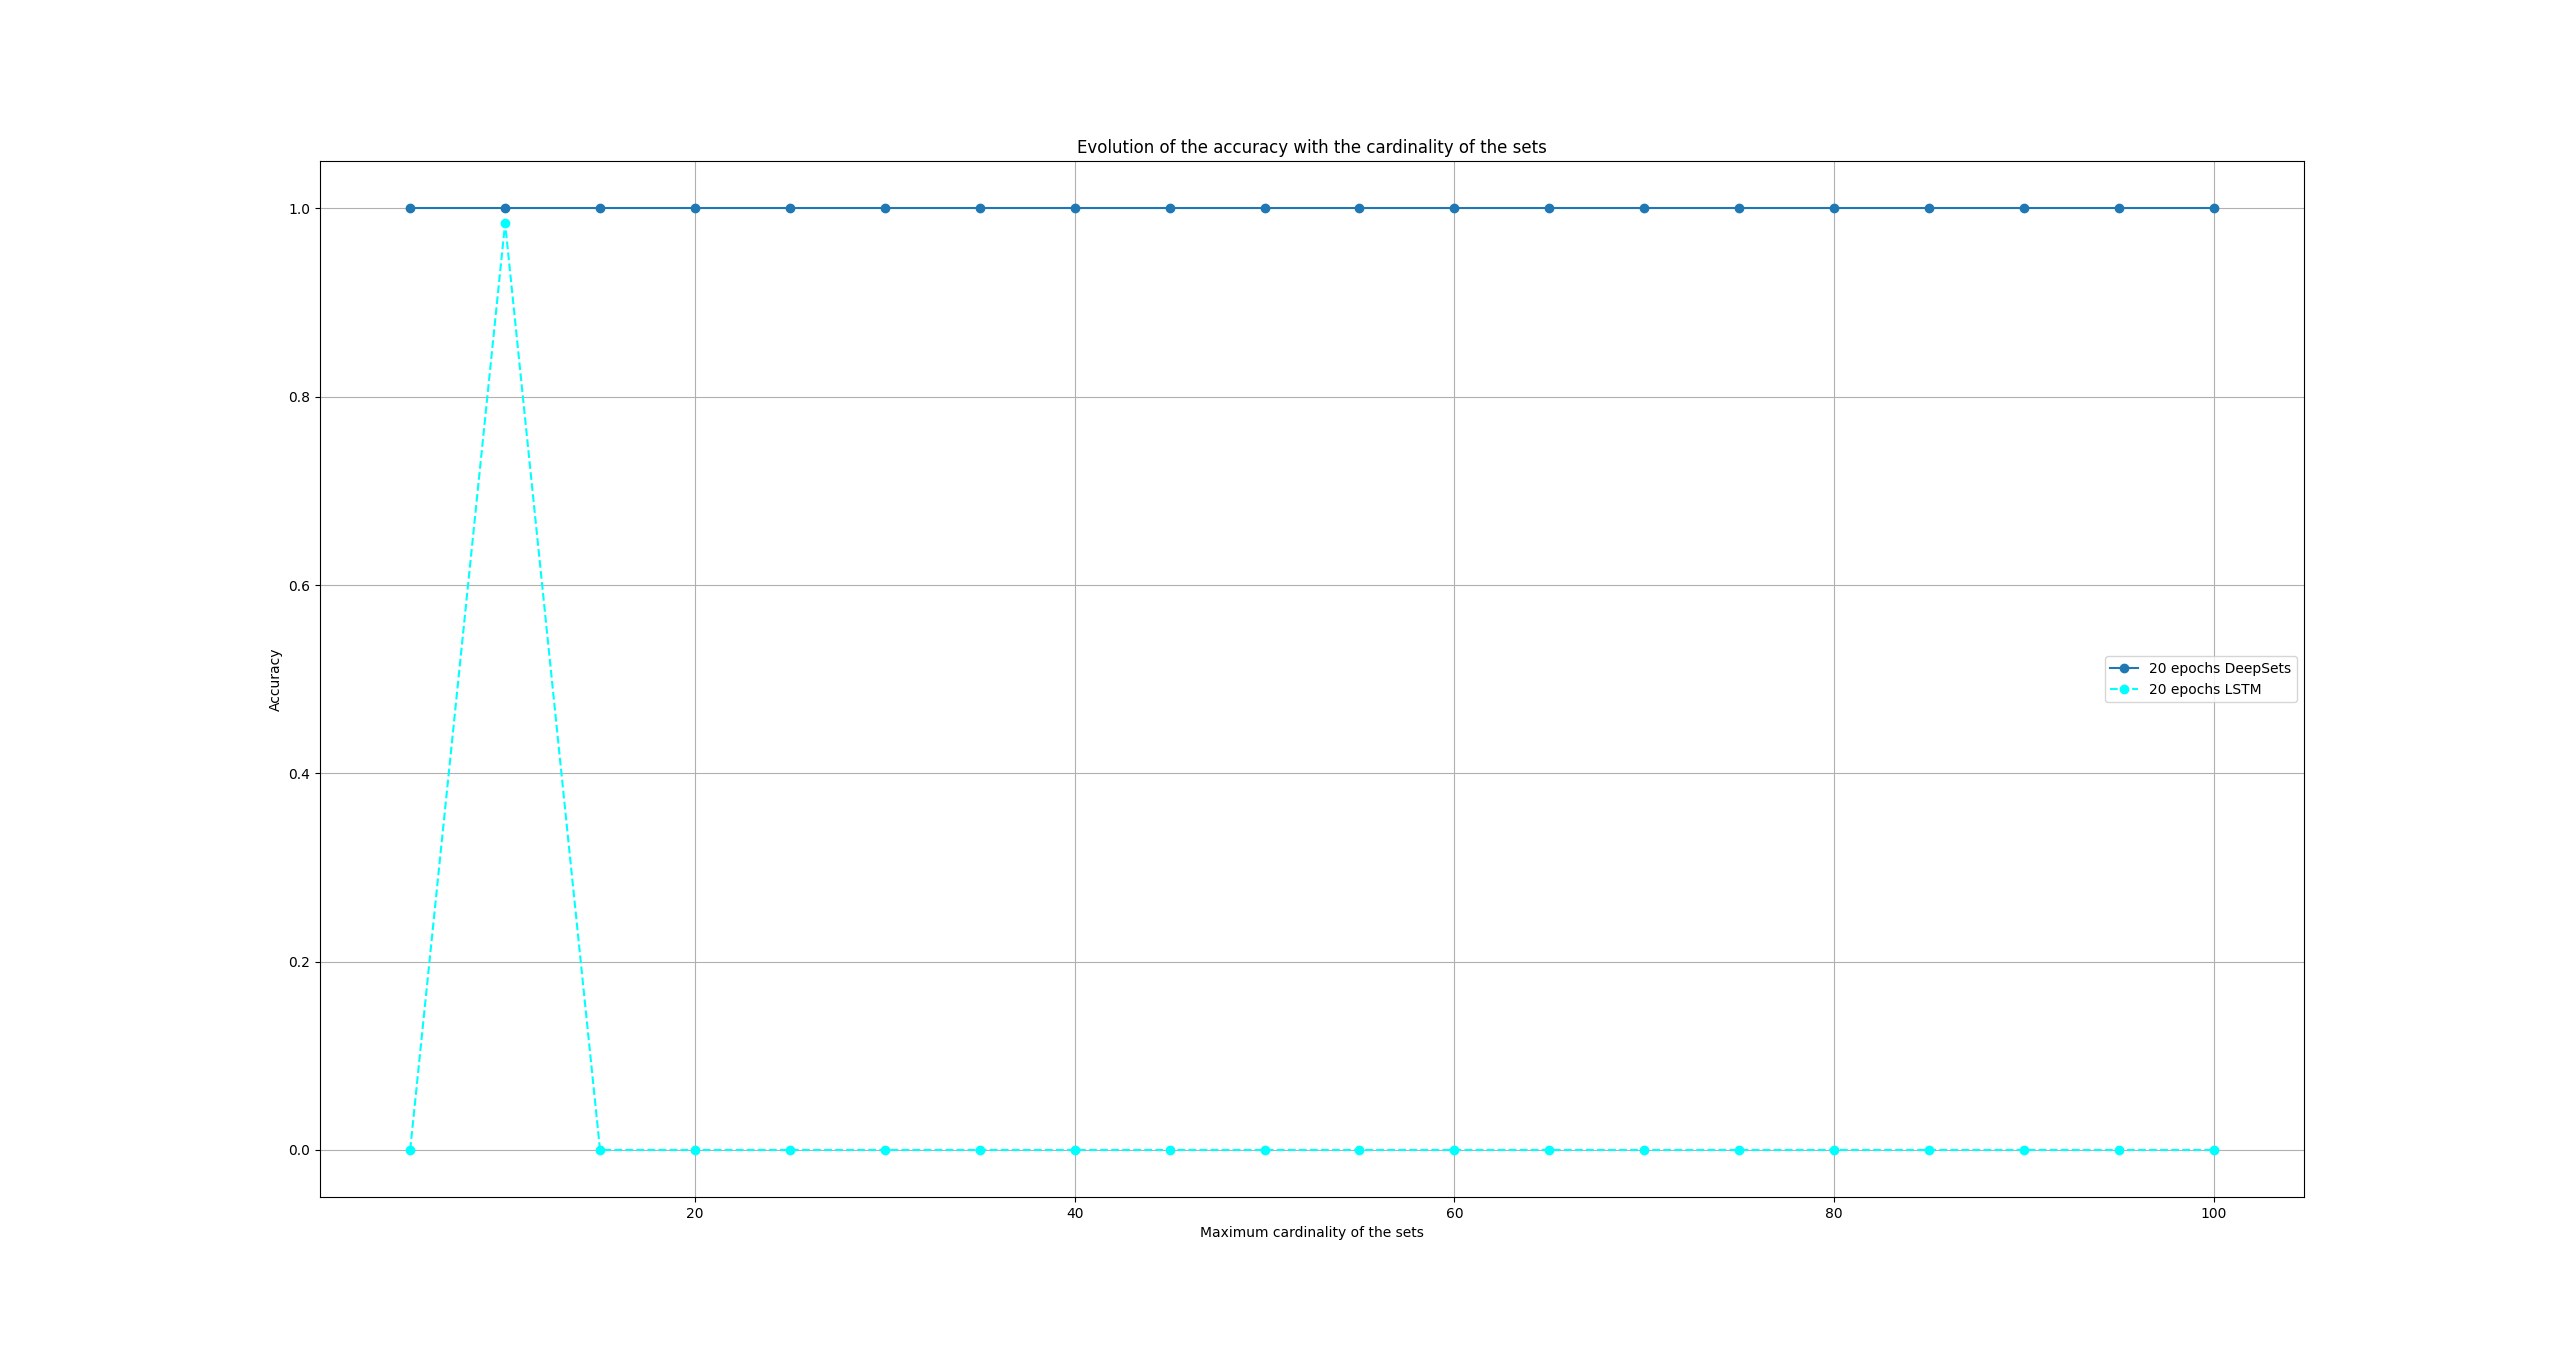
\includegraphics[width=1.\textwidth]{figures/deep_set_performances.png}
    \caption{Comparison of accuracies of the prediction of the sum over a set of integers with regard to the cardinality of the set. Deepset is able to generalize while LSTM fails (only rougly correct when summing 10 digits, in the regime it was trained).}
    \label{fig:performances_deepset_lstm}
\end{figure}



\begin{figure}[h]
    \centering
    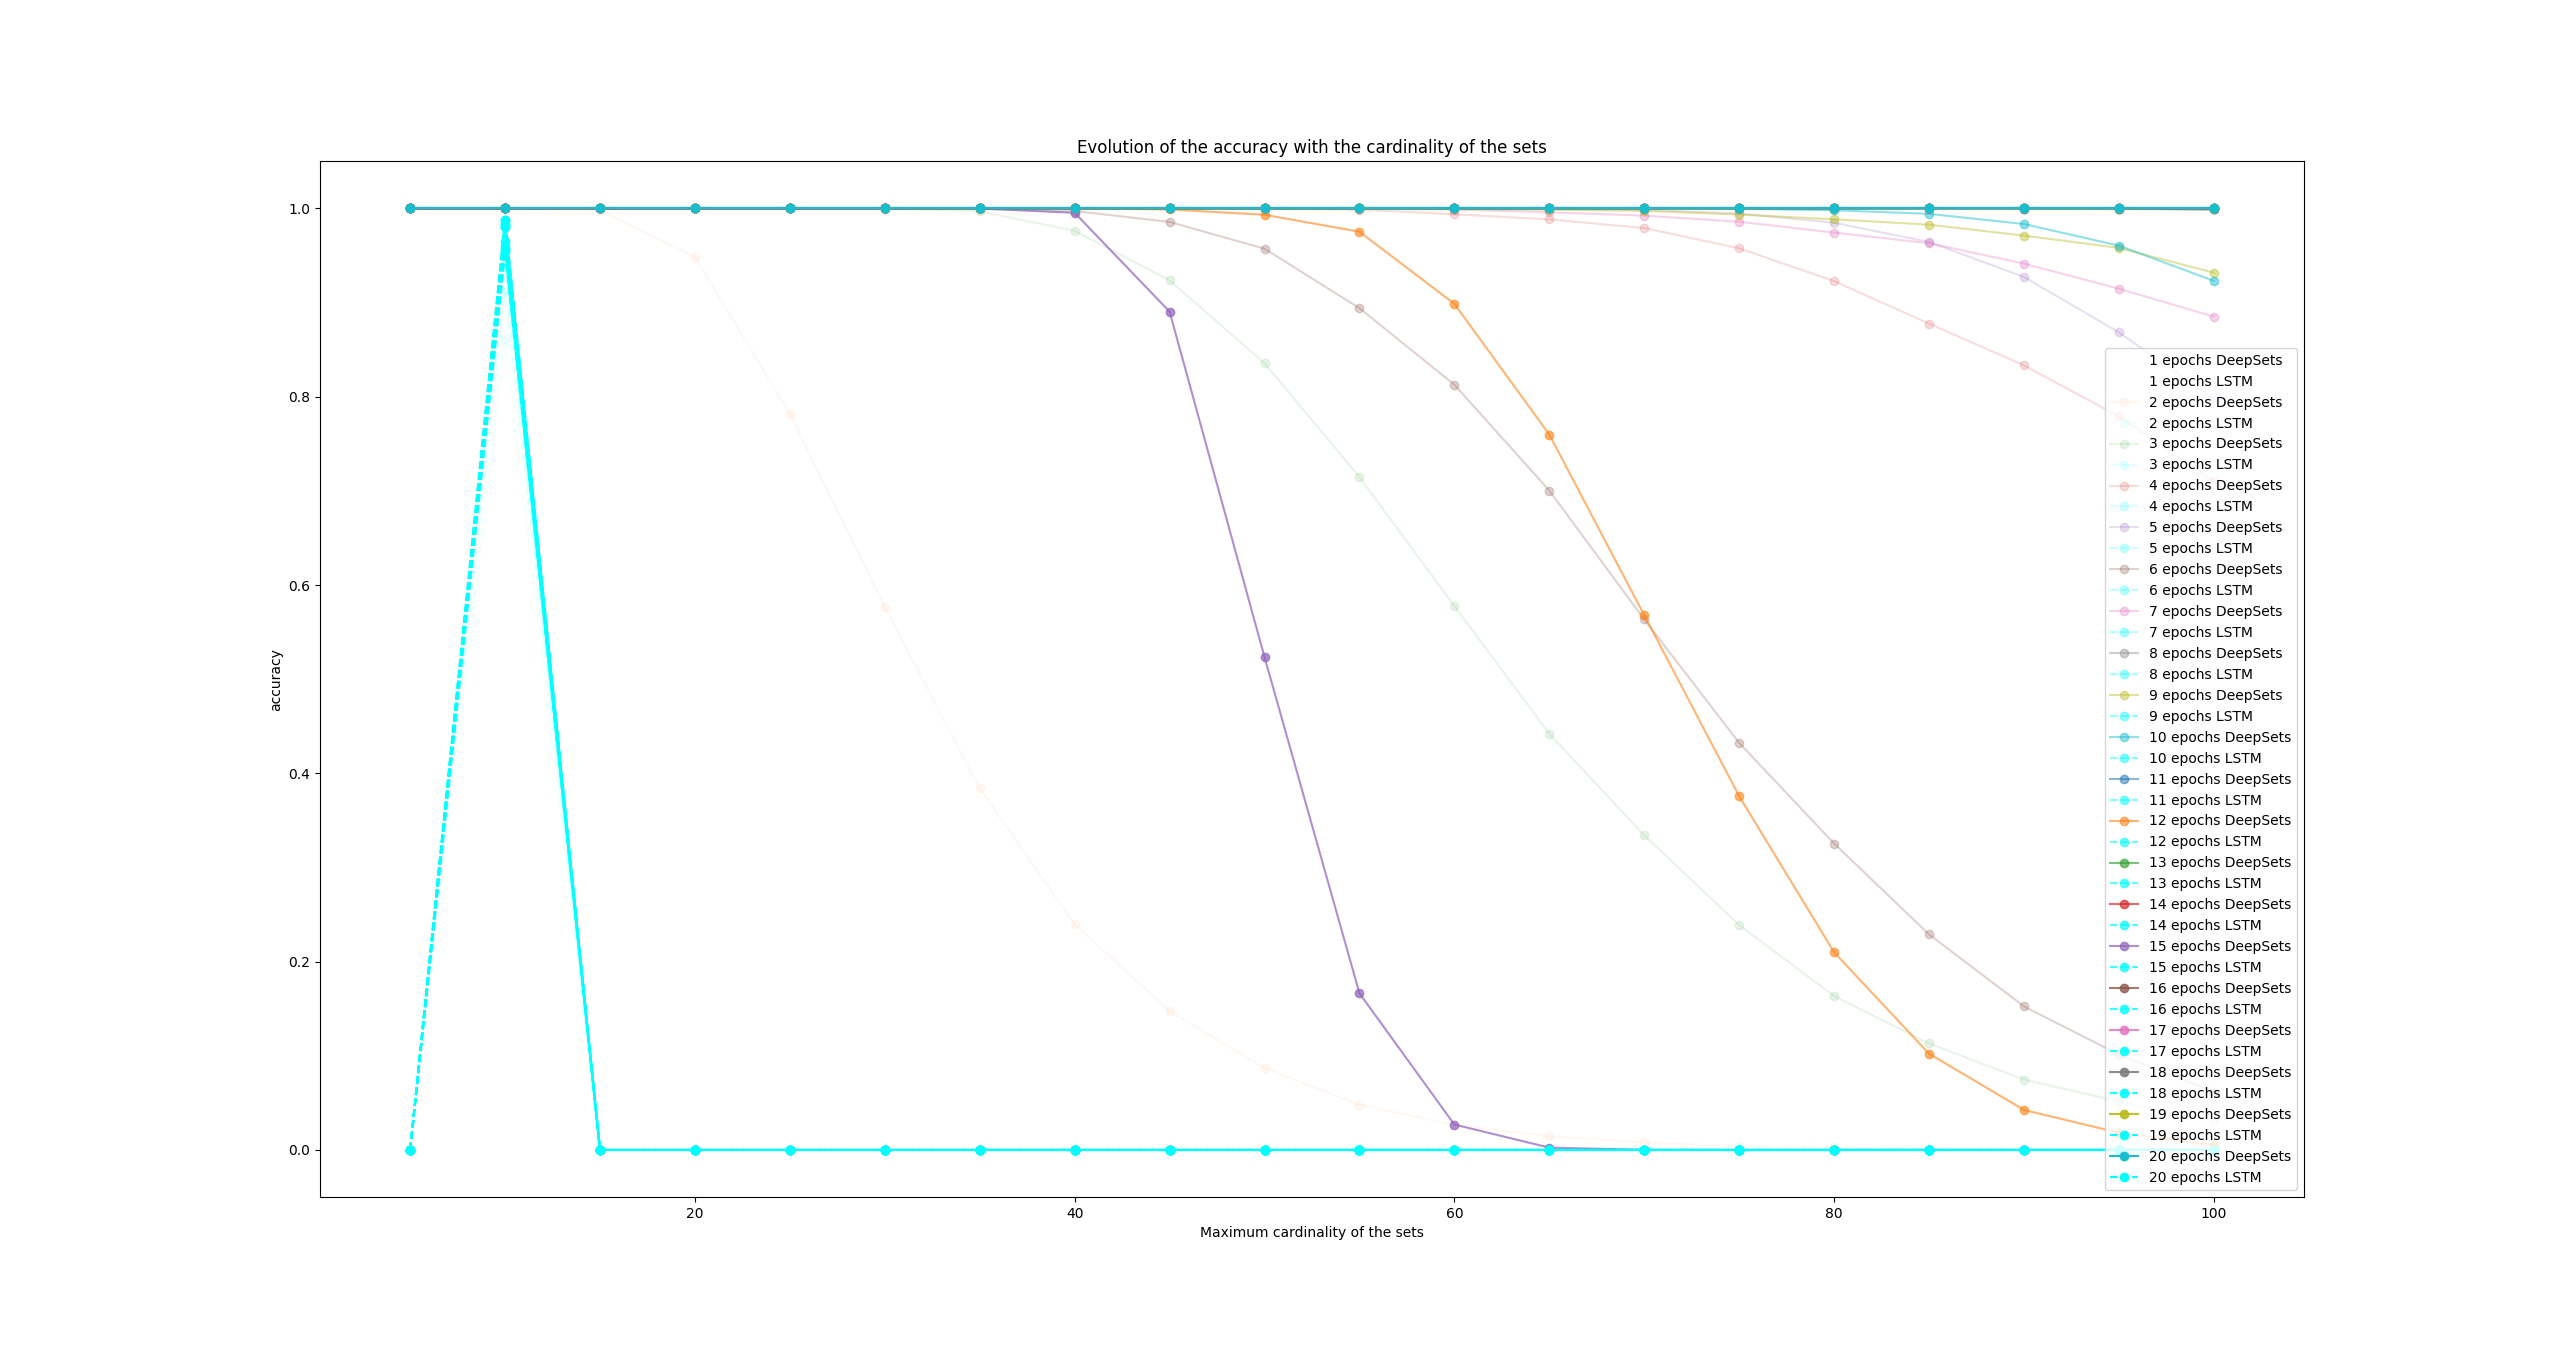
\includegraphics[width=1.\textwidth]{figures/deep_set_performances_evol.png}
    \caption{Evolution of the accuracies regarding cardinality during training}
    \label{fig:performances_deepset_lstm_evolution}
\end{figure}


% \bibliographystyle{plain}
% \bibliography{references}

\end{document}